\chapter{Project Description}
\label{chap:project_description}

\section{Requirements}
\label{sec:requirements}
\noindent In order fulfil the basic needs of any parking detection system, our proposed solution will feature the following: 
\begin{itemize}[noitemsep]
	\item Low power consumption – The system will focus on event-driven updates in order to conserve as much energy as possible and prolong time between sensor battery replacements.
	\item Ease of installation – With a wireless sensor network approach, this system will avoid cabling installation. Also, dynamic routing makes it possible to install sensors in a plug-and-play fashion.
	\item Reliability – The routing protocol focuses on reaching the control center keeping several alternate paths ready in case of connectivity loss.
	\item Error detection – By keeping track of each device's power level on every message, sensors running low on battery can be quickly identified and get a replacement before losing connectivity.
	\item Fast reaction times – The system will to notify parking status changes on time for the next car looking for a parking spot.
\end{itemize}

\section{Topology}
\label{sec:topology}
The two scenarios where this solution could be applied would be mainly in parking lots, and multi-story car parks, but also curb parking spaces.
In order to communicate the status of the parking spaces, wireless motes are programmed with one of three roles (see figure \ref{fig:topology}):
\begin{enumerate}
	\item Sensor - Node running on batteries equipped with a light sensor and encased in a protective shell that is fixed to the floor or pavement.
	It is responsible for monitoring parking space occupancy and inform its immediate Gateway of a status change.
	\item Gateway - Node connected to a power source in an elevated position (e.g. a street lamp). 
	It provides network access to the Sensors by forwarding their status messages towards the control center. 
	It also builds a distance-based routing table that consists of neighbor Gateway addresses and their distance to the control center.
	\item Central Station (CS) - Node connected to a computer or web server. This device will receive and process all status messages from every Gateway. 
	It also provides statistical information and GUI for the parking lot operator and information to be printed in an outdoor display for the drivers.
\end{enumerate}
The complete space detection and status forwarding is illustrated in figure \ref{fig:system_setup}.

\begin{figure}
    \centering
    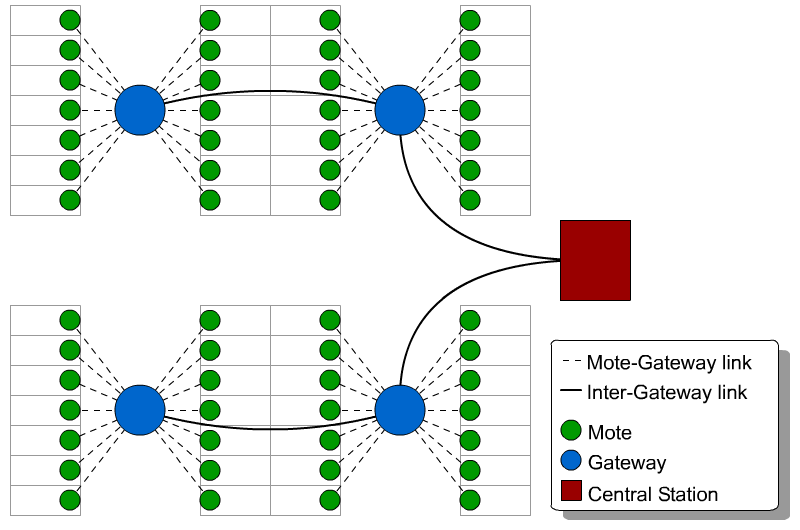
\includegraphics[width=15cm]{images/General_ParkingLotTopology.png}
	\vspace{-1.5em}
    \caption{Example topology of a small parking lot}
    \vspace{-1.5em}
    \label{fig:topology}
\end{figure}

\begin{figure}
    \centering
    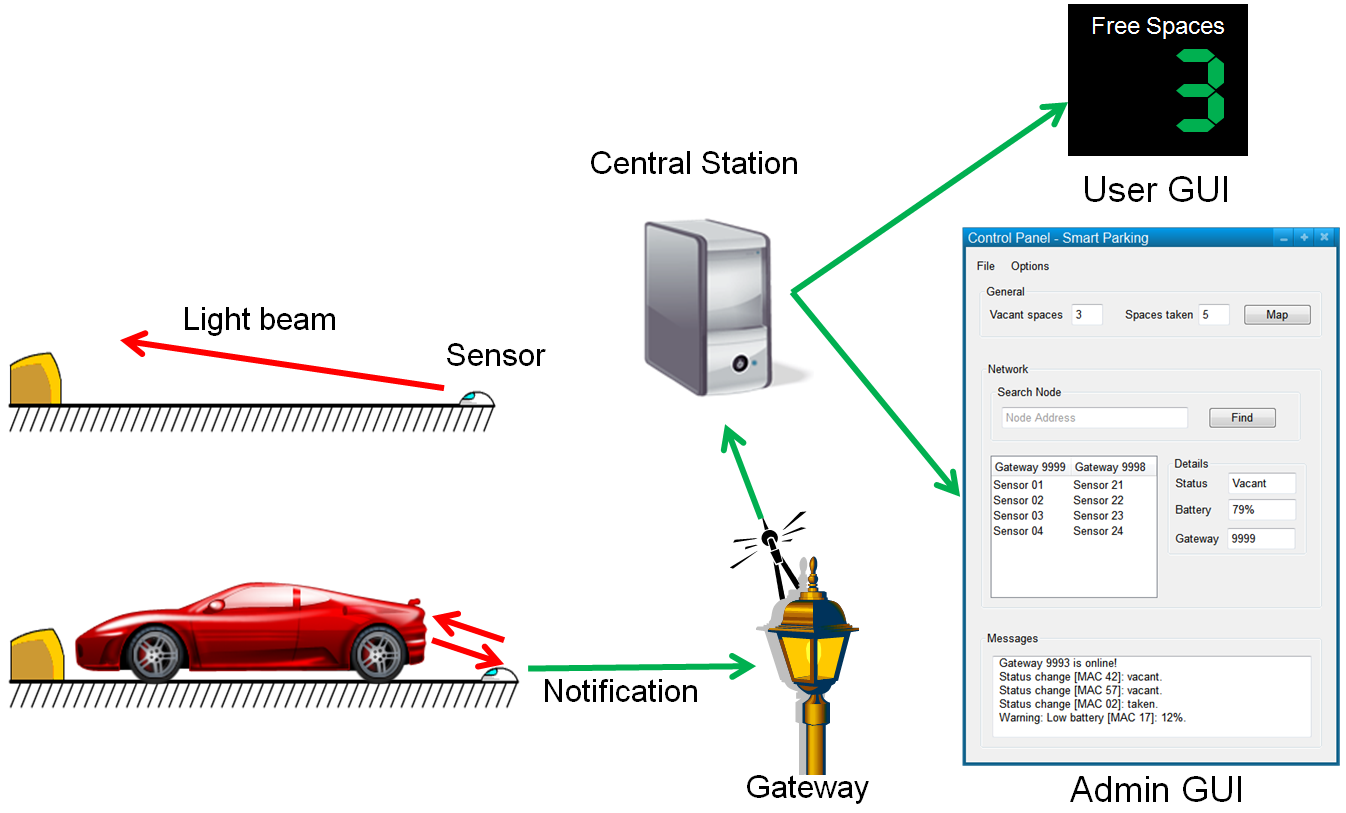
\includegraphics[width=15cm]{images/General_SpaceDetectionAndGUI.png}
	\vspace{-1.5em}
    \caption[System setup and vacant space detection]{System setup: Sensor motes are fixed onto the ground and detect if a car is using the parking space. 
	If the parking status changes, the Sensor notifies its Gateway. 
	The Gateway injects the notification into the network where it reaches the central station. 
	The central station publishes the information via an Admin GUI or a public display on the street.}
    \vspace{-1.5em}
    \label{fig:system_setup}
\end{figure}

\section{Routing}
\label{sec:routing}
The routing protocol proposed is dynamic and meant to ease installation in a plug-and-play fashion. 
The objectives of our implementation is to develop a simple, yet effective and fast route selection. 
It should provide quick reaction times and backup path switch-over in case of Gateway saturation or connectivity loss.
Lastly, it should allow new Sensors or Gateways to be added to the network with as little configuration effort as possible, if any.
We decided a protocol mix of Dijkstra and rumor routing could meet all these requirements.

\bigskip
\subsection{Rumor Routing}
\label{sec:rumor_routing}
In the original concept of query-based rumour routing \cite{rumor_routing_2002}, each node has a neighbor list and an events table. The events table contains forwarding information to all the events it knows. 
After a node witnesses an event, it sends a special long-lived packet to the network known as an agent.
The agent travels around the network hopping from node to node creating a path originating from the event.

Once there are events, agents and paths on the network, any node may send a query packet for a particular event into the network. 
If the query packet reaches a node who knows the route to the event (as told by a passing agent), it will forward the query. 
Otherwise, the query will be sent and propagated in a random direction until the query reaches a node with a route to the event. \\

\noindent Properties
\begin{itemize}[noitemsep]
	\item Power saving, improves network longevity.
	\item Robust in dealing node failure.
	\item Tunable, allow trade-off between setup overhead and delivery reliability.
\end{itemize}

\noindent Assumptions
\begin{itemize}[noitemsep]
	\item No coordinate system is available so location information is not known by nodes.
	\item Static topology.
\end{itemize}

\subsection{Dijkstra's algorithm for best path selection}
\label{sec:dijkstra}
This algorithm seeks the best path from a source node to a destination node in a given network.
It starts by assigning a tentative distance value to every node: set to zero for the initial node and to infinity for all other nodes.
Marks all nodes unvisited. Sets the initial node as current. Creates a set of the unvisited nodes called the unvisited set consisting of all the nodes.

Once all these initial settings are done, an iterative process begins in which each node is evaluated for the shortest distance:
\begin{enumerate}[noitemsep]
	\item For the current node, all of its unvisited neighbors are evaluated and their tentative distances are calculated.
	\item It then compares the newly calculated tentative distance to the current assigned value and assign the smaller one. 
	\item When all of neighbors of the current node has been evaluated, the current node is marked as visited and removed from the unvisited set. 
	\item If the destination node has been marked visited or if the smallest tentative distance among the nodes in the unvisited set is infinity, the algorithm stops.
	\item The next step is to take the unvisited node with the smallest tentative distance as the new "current node" and go back to the first step.
\end{enumerate}

\noindent Properties
\begin{itemize}[noitemsep]
	\item Clever way to use cost/distance to select a path.
	\item Focused in looking for one path only (i.e. the algorithm must be run on every device).
	\item Looking for the shortest path by flooding consumes a lot of energy.
	\item Flooding increases the chance of collision.
\end{itemize}

\subsection{The rumor-Dijkstra hybrid}
\label{sec:hybrid}
As we have seen, rumor routing and Dijkstra's algorithm have attractive properties that could provide advantageous to our purposes. 
In order to provide a practical, simple and fast solution we had to mix the most convenient features to our topology :

\begin{itemize}[noitemsep]
	\item After booting, a new node will broadcast a special packet called GW\_REQ (meaning "Gateway request". See section \ref{sec:packet_format} for more details on packet types)
	\item Every Gateway that receives a GW\_REQ, must reply with an UPDATE packet, which contains its MAC address and its distance to the CS.
	\item The new node then waits for all UPDATE packets. From all replies, 5 best neighboru nodes are selected and inserted into the routng table.
	\item In the case of Sensors, the metric is the Received Signal Strength Indicator (RSSI; the higher, the better) and for Gateways is distance to the central station (the lower, the better).
	\item After a Gateway reads the distance of an UPDATE, it also checks the signal strength of the packet and adds a weight depending on the RSSI value:\\
			\centerline{+1 if \(>\) 0 , +2 if \(>\) -15, +3 if \(\leq\) -15}. 
	\item The replies with the five best metrics are put in the routing table. In the case of Gateways, the best distance (+ RSSI weight) in the table becomes its own distance. If own distance is changed, that means that there was a change in topology so the node must broadcast the UPDATE message to notify other nodes in the vicinity. This ensures that every significant change of topology instantly spreads through the network. 
	The device can then begin with the tasks specific to its role (Gateway or Sensor).
	\item If there was no response at all, the device will repeat the process over and over again sending GW\_REQ packets until it receives an UPDATE.
\end{itemize}

\begin{figure}
    \centering
    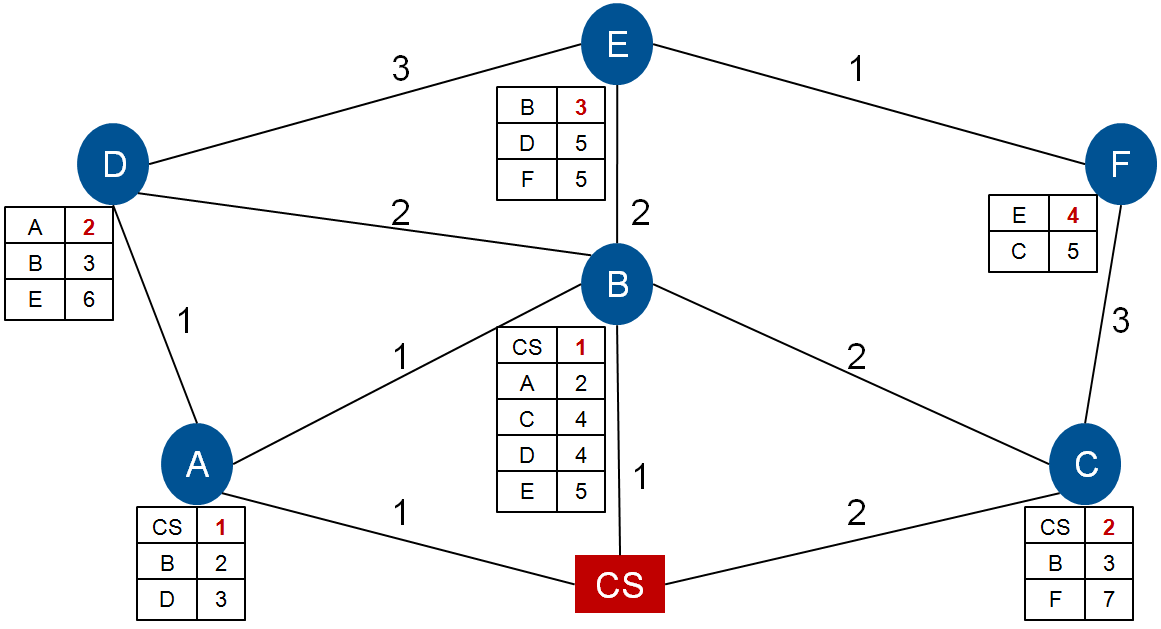
\includegraphics[width=15cm]{images/Example_Routing.png}
	\vspace{-1.5em}
    \caption[Best path discovery example]{Example of best path discovery. 
	The number in the lines connecting the nodes are the weights taken from the RSSI values of each link: 1 if \(>\) 0 , 2 if \(>\) -15, 3 if \(\leq\) -15.
	The blue circles represent Gateways and the red square is the central station (CS).
	Each node keeps a table with five of its neighbors with the shortest distance to the CS.
	The red number is the distance each node reports in UPDATE packets.}
    \vspace{-1.5em}
    \label{fig:routing}
\end{figure}

In contrast to the original rumor routing concept, the hybrid does not consider events as information source or an agent traversing the network. 
Instead, it makes emphasis on routing by exchanging information with neighbors only. 
Their only interest is about their distance to the central station and/or signal strength.

Also, instead of running a Dijkstra algorithm to check every single node for their link cost and update it after every calculation, we took the concept of cost and a step-wise evaluation of the best path to a specific node. 
This process happens locally on every node and this information will be exchanged with neighbors only. 

UPDATE packets are sent in two situations: As a response on GW\_REQ packet during network discovery (see section \ref{sec:network_discovery} for more on the network discovery), or if its best route changed.
If best route is changed, that means that the information about distance to the CS that neighbouring nodes have through this node are not up to date anymore. Because of this, the node sens an UPDATE packet to its neighbours, reporting that the path is better or worse. If this also has an effect on the best route of the next node, the same procedure happens on the next node. If a change has no effect on a next nodes own distance, the next node stays silent because from here all the data is up to date. In this way the information spreads as far as it has an effect and entire network stays up to date with as little overhead as possible.